\begin{figure}[htbp]
			\centering
			\resizebox{\textwidth}{!}{%
				\begin{tikzpicture}[
					scale=0.95,
					>=latex,
					trave/.style={line width=1.2pt},
					carico/.style={black, line width=0.6pt},
					forza/.style={black, line width=1pt},
					diagT/.style={black, line width=0.8pt},
					diagM/.style={black, line width=0.8pt},
					hatch/.style={gray!50, line width=0.3pt},
					quota/.style={black, line width=0.4pt},
					fibre/.style={gray!70, line width=0.3pt},
					]
					
					% ── Parametri dei vincoli (convenzione C06/C07) ──
					\def\tw{0.15}    \def\thR{0.28}   \def\rn{0.06}
					\def\rw{0.05}    \def\bw{0.09}    \def\gw{0.22}
					\def\hh{0.10}
					
					% ── Geometria del problema ──
					\def\Lell{4}                            % lunghezza trave ℓ
					\pgfmathsetmacro{\xA}{0}
					\pgfmathsetmacro{\xMid}{0.5*\Lell}      % mezzeria ℓ/2 = 2
					\def\yqi{-0.80}                         % y delle quote sotto la trave
					\def\ylab{-3.30}                        % y delle etichette di pannello
					
					% ── Parametri del carico distribuito ──
					\def\pgap{0.10}                         % gap fra trave e base del riquadro
					\def\php{1.0}                          % altezza del riquadro
					\pgfmathsetmacro{\pBase}{\pgap}         % base del riquadro: y = 0,05
					\pgfmathsetmacro{\pTop}{\pgap+\php}     % cima del riquadro: y = 0,45
					
					% =========================================================
					% PANNELLO (a) — Schema statico
					% =========================================================
					\begin{scope}[xshift=0cm]
						
						% ── Trave ──
						\draw[trave] (0,0) -- (\Lell,0);
						
						% ── Fibra inferiore (tratteggio sotto la trave) ──
						\draw[fibre, dashed] (0, -0.1) -- (\Lell, -0.1);
						
						% ── Cerniera in A ──
						\draw[thick] (0,0) -- (-\tw,-\thR) -- (\tw,-\thR) -- cycle;
						\draw[thick] (-\gw,-\thR) -- (\gw,-\thR);
						\foreach \x in {-0.16,-0.08,0,0.08,0.16}
						\draw[thin] (\x,-\thR) -- ++(-0.07,-\hh);
						
						% ── Carrello verticale in B ──
						\draw[thick] (\Lell,0) -- (\Lell-\tw,-\thR) -- (\Lell+\tw,-\thR) -- cycle;
						\draw[thick] (\Lell-\bw,-\thR-\rw-0.01) circle (\rw);
						\draw[thick] (\Lell+\bw,-\thR-\rw-0.01) circle (\rw);
						\draw[thick] (\Lell-\gw,-\thR-2*\rw-0.04) -- (\Lell+\gw,-\thR-2*\rw-0.04);
						\foreach \x in {-0.16,-0.08,0,0.08,0.16}
						\draw[thin] (\Lell+\x,-\thR-2*\rw-0.04) -- ++(-0.07,-\hh);
						
						% ── Anellini bianchi sui perni ──
						\draw[thick, fill=white] (0,0) circle (\rn);
						\draw[thick, fill=white] (\Lell,0) circle (\rn);
						
						% ── Etichette A, B ──
						\node[above left=-2pt,  font=\small] at (0,0)      {$A$};
						\node[above right=-2pt, font=\small] at (\Lell,0)  {$B$};
						
						% ── Carico distribuito p̄ sopra la trave ──
						% Bordi orizzontali del riquadro (la chiusura laterale la fanno le frecce sui bordi)
						\draw[carico] (0,\pBase) -- (\Lell,\pBase);
						\draw[carico] (0,\pTop)  -- (\Lell,\pTop);
						% Frecce equispaziate, code sul bordo superiore, punte sul bordo inferiore;
						% includono i due bordi laterali x=0 e x=ℓ
						\foreach \x in {0, 0.50, 1.00, ..., 4.00} {
							\draw[->, carico] (\x, \pTop) -- (\x, \pBase);
						}
						% Etichetta p̄ sopra il riquadro, a lato (verso destra)
						\node[above, font=\small] at (\Lell/2, \pTop) {$\bar{p}$};
						
						
						% ── Quota ℓ sotto la trave ──
						\draw[<->, quota] (0,\yqi) -- (\Lell,\yqi);
						\draw[quota] (0,\yqi+0.07)     -- (0,\yqi-0.07);
						\draw[quota] (\Lell,\yqi+0.07) -- (\Lell,\yqi-0.07);
						\node[above, font=\small] at (\xMid, \yqi-0.04) {$\ell$};
						
						% Etichetta pannello (a)
						\node[font=\small] at (0.5*\Lell, 0.4*\ylab) {(a)};
						
					\end{scope}
					
					% =========================================================
					% PANNELLO (b) — Diagramma di T(z)
					% =========================================================
					\begin{scope}[xshift=5.5cm]
						
						% ── Trave (clone) ──
						\draw[trave] (0,0) -- (\Lell,0);
						
						% ── Vincoli (clone) ──
						\draw[thick] (0,0) -- (-\tw,-\thR) -- (\tw,-\thR) -- cycle;
						\draw[thick] (-\gw,-\thR) -- (\gw,-\thR);
						\foreach \x in {-0.16,-0.08,0,0.08,0.16}
						\draw[thin] (\x,-\thR) -- ++(-0.07,-\hh);
						\draw[thick] (\Lell,0) -- (\Lell-\tw,-\thR) -- (\Lell+\tw,-\thR) -- cycle;
						\draw[thick] (\Lell-\bw,-\thR-\rw-0.01) circle (\rw);
						\draw[thick] (\Lell+\bw,-\thR-\rw-0.01) circle (\rw);
						\draw[thick] (\Lell-\gw,-\thR-2*\rw-0.04) -- (\Lell+\gw,-\thR-2*\rw-0.04);
						\foreach \x in {-0.16,-0.08,0,0.08,0.16}
						\draw[thin] (\Lell+\x,-\thR-2*\rw-0.04) -- ++(-0.07,-\hh);
						\draw[thick, fill=white] (0,0) circle (\rn);
						\draw[thick, fill=white] (\Lell,0) circle (\rn);
						
						% ── Etichette A, B ──
						\node[above left=-2pt,  font=\small] at (0,0)      {$A$};
						\node[above right=-2pt, font=\small] at (\Lell,0)  {$B$};
						
						% ── Tacca verticale in mezzeria z₀ = ℓ/2 ──
						\draw[forza] (\xMid, -0.10) -- (\xMid, 0.10);
						% Etichetta ℓ/2 sotto la trave, vicina alla tacca
						\node[above, font=\footnotesize] at (\xMid,0.04) {$\ell/2$};
						
						% ── Diagramma T(z) ──
						\def\sT{0.45}
						\pgfmathsetmacro{\Tpos}{ 0.5*\Lell*\sT}    % T(A) = +p̄ℓ/2 → +0.70
						\pgfmathsetmacro{\Tneg}{-0.5*\Lell*\sT}    % T(B) = -p̄ℓ/2 → -0.70
						
						% Hatching verticale dall'asse al diagramma — attraversa lo zero in ℓ/2
						% Parametrizzo con t = x/ℓ ∈ [0,1]; h(t) = (1 - 2t)·Tpos
						\foreach \x in {0.20, 0.40, ..., 3.80} {
							\pgfmathsetmacro{\t}{\x/\Lell}
							\pgfmathsetmacro{\h}{(1 - 2*\t)*\Tpos}
							\draw[hatch] (\x, 0) -- (\x, \h);
						}
						
						% Bordo del diagramma — un solo segmento più due verticali di chiusura
						\draw[diagT]
						(0, 0) -- (0, \Tpos)             % verticale in A
						-- (\Lell, \Tneg)                % lineare da +T_pos in A a -T_pos in B
						-- (\Lell, 0);                   % verticale di chiusura in B
						
						% Segni cerchiati nei due triangoli
						% Triangolo positivo (sopra, sinistra): centroide a (ℓ/3, T_pos/3)
						\node[font=\small] at ({\Lell/6}, {\Tpos/3}) {$\boldsymbol{\oplus}$};
						% Triangolo negativo (sotto, destra): centroide a (2ℓ/3, T_neg/3)
						\node[font=\small] at ({5*\Lell/6}, {\Tneg/3})	{$\boldsymbol{\ominus}$};
						
						% Valori notevoli (senza segno, come da convenzione)
						\node[left, font=\small] at (0, \Tpos) {$\tfrac{\bar{p}\ell}{2}$};
						\node[right, font=\small] at (\Lell, \Tneg)	{$\tfrac{\bar{p}\ell}{2}$};
						
						% Etichetta pannello (b)
						\node[font=\small] at (0.5*\Lell, 0.4*\ylab) {(b)};
						
					\end{scope}
					
					% =========================================================
					% PANNELLO (c) — Diagramma di M(z)
					% =========================================================
					\begin{scope}[xshift=11.0cm]
						
						% ── Trave (clone) ──
						\draw[trave] (0,0) -- (\Lell,0);
						
						% ── Vincoli (clone) ──
						\draw[thick] (0,0) -- (-\tw,-\thR) -- (\tw,-\thR) -- cycle;
						\draw[thick] (-\gw,-\thR) -- (\gw,-\thR);
						\foreach \x in {-0.16,-0.08,0,0.08,0.16}
						\draw[thin] (\x,-\thR) -- ++(-0.07,-\hh);
						\draw[thick] (\Lell,0) -- (\Lell-\tw,-\thR) -- (\Lell+\tw,-\thR) -- cycle;
						\draw[thick] (\Lell-\bw,-\thR-\rw-0.01) circle (\rw);
						\draw[thick] (\Lell+\bw,-\thR-\rw-0.01) circle (\rw);
						\draw[thick] (\Lell-\gw,-\thR-2*\rw-0.04) -- (\Lell+\gw,-\thR-2*\rw-0.04);
						\foreach \x in {-0.16,-0.08,0,0.08,0.16}
						\draw[thin] (\Lell+\x,-\thR-2*\rw-0.04) -- ++(-0.07,-\hh);
						\draw[thick, fill=white] (0,0) circle (\rn);
						\draw[thick, fill=white] (\Lell,0) circle (\rn);
						
						% ── Etichette A, B ──
						\node[above left=-2pt,  font=\small] at (0,0)      {$A$};
						\node[above right=-2pt, font=\small] at (\Lell,0)  {$B$};
						
						% ── Tacca verticale in mezzeria z₀ = ℓ/2 ──
						\draw[forza] (\xMid, -0.10) -- (\xMid, 0.10);
						
						% ── Diagramma M(z) ──
						% Scala: 1 (p̄·ℓ²) = \sM unità di figura  (M positivo SOTTO l'asse)
						% M(z) = (p̄/2)·z·(ℓ-z), parabolico, max p̄ℓ²/8 in mezzeria
						\def\sM{0.50}
						\pgfmathsetmacro{\Mmax}{-(\Lell*\Lell/8)*\sM}   % M(ℓ/2) = +p̄ℓ²/8 → -0.80 (sotto)
						
						% Hatching verticale: dall'asse al diagramma
						\foreach \x in {0.20, 0.40, ..., 3.80} {
							\pgfmathsetmacro{\h}{(\x*(\Lell-\x)/(\Lell*\Lell/4))*\Mmax}
							\draw[hatch] (\x, 0) -- (\x, \h);
						}
						
						% Bordo del diagramma — parabola campionata a 21 punti (passo 0,20)
						\draw[diagM]
						(0.00, 0)
						\foreach \x in {0.20, 0.40, ..., 3.80} {
							-- ({\x}, {(\x*(\Lell-\x)/(\Lell*\Lell/4))*\Mmax})
						}
						-- (\Lell, 0);
						
						% Valore notevole — etichetta sotto il vertice della parabola
						\node[above, font=\small] at (\xMid, \Mmax-0.04){$\tfrac{\bar{p}\ell^2}{8}$};
						
						% Etichetta ℓ/2 sotto la trave, vicina alla tacca
						\node[above, font=\small] at (\xMid,0.04) {$\ell/2$};
						
						% Etichetta pannello (c)
						\node[font=\small] at (0.5*\Lell, 0.4*\ylab) {(c)};
						
					\end{scope}
					
				\end{tikzpicture}
			}
			\caption{Trave appoggiata con carico uniformemente distribuito
				$p(z) = \bar{p}$ (verso il basso) su tutta la trave:
				(a)~schema strutturale;
				(b)~diagramma del taglio $T(z)$, lineare decrescente, con
				valori $\bar{p}\ell/2$ in $A$ e $-\bar{p}\ell/2$ in $B$
				e annullamento in mezzeria $z_0 = \ell/2$;
				(c)~diagramma del momento flettente $M(z)$, parabolico
				con concavità verso l'alto, nullo agli estremi e massimo
				$\bar{p}\ell^2/8$ in mezzeria, in corrispondenza del punto
				dove il taglio si annulla.}
			\label{fig:stat_trasv_iso_02}
		\end{figure}
